\documentclass[10pt,a4paper]{article}
\usepackage[utf8]{inputenc}
\usepackage[catalan]{babel}
\usepackage[margin=2.5cm]{geometry}
\usepackage[procnames]{listings}
\usepackage{graphicx}
\usepackage{titling}
\usepackage{fancyhdr}
\usepackage{float}
\usepackage{amsmath}
\usepackage{enumitem}
\usepackage{hyperref}
\graphicspath{{images/}}
\usepackage[x11names]{xcolor}
\usepackage{listings}
\usepackage{longtable}
\usepackage{subfig}
\usepackage{hyperref}
 
\title{XtiSpd: Comunicació amb llum visible}
\author{Sudan Wu}
\date{\today}


\pagestyle{fancy}
\fancyhf[lh]{XtiSpd: Treball}
\fancyhf[rh]{\theauthor}
\fancyhf[cf]{\thepage}

\begin{document}

\begin{titlepage}
    \begin{center}
        
\includegraphics[height=1.8cm]{logoUdG}\\\vfill
    \end{center}
    \center
    {\huge \bfseries Xarxes troncals i Serveis públics de dades}\\[0.5cm]
    {\Huge \bfseries Visible light communication} \\[0.5cm]
    {\Huge \bfseries (VLC)} \\[0.5cm]

    \vfill
    \begin{center} \large
        {Sudan Wu, sudan88792@gmail.com} \\[0.25cm]
        {\today}\\ [1cm]
    \end{center}

\end{titlepage}

\tableofcontents

\clearpage

\section{Que és la Comunicació amb llum visible}


hhhjhlkjgkjh

- teoria de llum (laser + aigua)
- estructura de la fibra, gruxut
- comunicarse atraves de la llum

- usuarios que utilizan opticas
- fabriques mundials
- processos de fer
- el preu
- 1841 fanshe
- cristal

\subsection*{Introducció}
\addcontentsline{toc}{subsection}{Introducció}
La comunicació amb llum visible (coneguda com a VLC, acrònim en anglès de "visible light communication") és un mitjà transmissor de dades que utilitza la llum entre 400 i 800 THz (780-375 nm). VLC és un subconjunt de tecnologies de comunicacions òptiques sense fil.



\begin{center}
    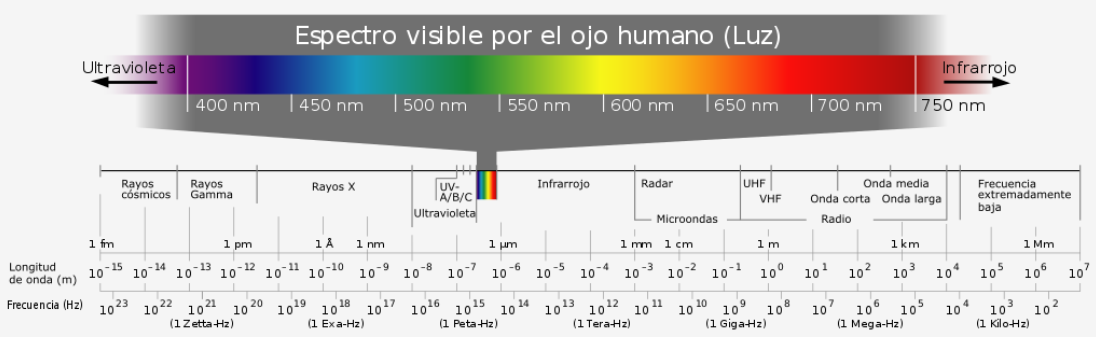
\includegraphics[height=3.8cm]{llumVisible.png}\\\vfill
\end{center}

La tecnologia  VLC utilitza llums fluorescents (làmpades normals, no necessita dispositius especials) per transmetre senyals a una velocitat de 10 kbit/s, o LEDs que pot assolir velocitats de fins a 500 Mbit/s. RONJA aconsegueix assolir una velocitat d'Ethernet completa (10 Mbit/s) sobre la mateixa distància gràcies a una òptica més gran i LED més potents.

La VLC pot ser utilitzada com un mitjà transmissor de computació ubiqua, atès que els dispositius que produeixen llum (làmpades d'interior exterior, televisors, senyals de trànsit, lluminosos comercials, fars de vehicles3) utilitzats a tot arreu, es poden aprofitar. El fer ús de la llum visible és també menys perillosa per a aplicacions que utilitzen una gran potència, ja que, els éssers humans poden percebre i protegirse-se del dany que pugui ocasionar-los.




\subsection*{El mercat del visible Light communication}
\addcontentsline{toc}{subsection}{El mercat del visible Light communication}

\subsubsection*{Visió general del mercat de la Visible Light communication}
Els sistemes de comunicació de llum visible (VLC) s'utilitzen per crear xarxes de comunicació d'alta velocitat, segures i biològicament amigables que permeten la formació i l'expansió d'aplicacions informàtiques unificades. Aquests sistemes utilitzen longituds d'ona de llum modificades emeses per una varietat de fonts, com ara il·luminació exterior i interior, senyals, taulers de visualització, televisors, pantalles d'ordinador, càmeres digitals i càmeres digitals en telèfons mòbils amb finalitats de comunicació, principalment mitjançant l'ús de díodes emissors de llum. (LEDs).

\begin{center}
    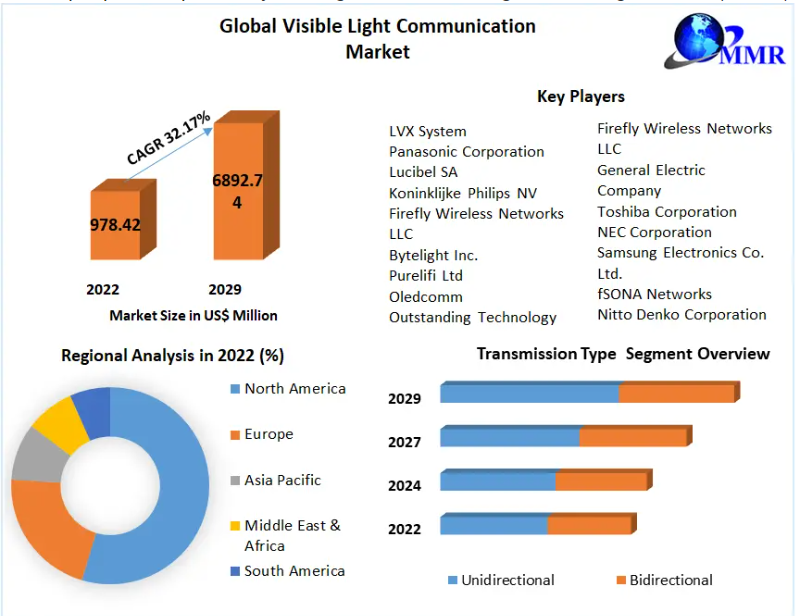
\includegraphics[height=5.8cm]{visiogeneralVLC.png}\\\vfill
\end{center}



Altres subconjunts de tecnologies de comunicació òptiques sense fil són:
\begin{itemize}
    \item Infraroig (IR): Encara que no és visible per a l'ull humà, la llum infraroja s'utilitza en diverses tecnologies sense fil, com ara els controls remots, els dispositius de comunicació a curta distància i les transmissions de dades sense fil en alguns contextos.
    \item Comunicació Òptica d'Espai Lliure (FSO): Aquesta tecnologia utilitza feixos de llum làser per a la transmissió de dades sense cables a través de l'espai lliure, com ara entre dos edificis. És especialment útil en línies de vista directa sense obstruccions.
    \item Comunicació Òptica Inalàmbrica (OWC): Aquesta tecnologia inclou diverses formes de transmissió de dades sense fil a través de llum òptica, incloent l'ús de làsers i LED.
    \item Comunicació Òptica en Entorns Controlats: En alguns entorns, com ara entorns d'oficines o fàbriques, es poden utilitzar sistemes d'òptica sense fil per a la transmissió de dades en lloc de les tecnologies tradicionals sense fil.
\end{itemize}

cada tecnologia té les seves pròpies aplicacions, avantatges i desavantatges. La selecció de la tecnologia òptica sense fil adequada depèn dels requisits específics de l'aplicació i les condicions de l'entorn.


La comunicació de llum visible exclourà la necessitat d'altres tecnologies sense fil, com ara infrarojos (IR), Bluetooth i Wi-Fi que emeten interferències electromagnètiques (EMI) i ones de RF que són perjudicials no només per als instruments/dispositius, sinó també per als humans. Així, el mercat es troba en una fase de creixement exponencial i es calcula que creixerà amb un CAGR elevat de xx.xx\% a tot el món durant el període de previsió.


L'augment de la població i els vehicles a la carretera creant enormes reptes per a la gestió del trànsit. El volum de dades transmeses a través de Wi-Fi al carrer no és suficient ni segur per a una gestió eficient. D'altra banda, en la gestió del trànsit, una aplicació encoratjadora per a VLC és la comunicació de vehicle a vehicle i de vehicle a infraestructura.

Com que els semàfors utilitzen il·luminació LED, és una oportunitat emergent en els sistemes de gestió del trànsit, com ara els semàfors i els senyals de trànsit amb VLC. Per exemple, els llums del carrer que s'interconnecten amb el telèfon intel·ligent equipat amb VLC d'un caminant poden controlar el trànsit de vehicles, permetent als caminants creuar un carrer.

La majoria dels fars i fars posteriors dels cotxes s'estan substituint per LED. VLC pot transformar aquests LED per a la comunicació de cotxe a cotxe. Aquesta influència pot millorar els sistemes anticolisió i permetre l'intercanvi d'informació entre vehicles. Per contra, l'eficiència d'aquests sistemes de trànsit intel·ligents es pot veure afectada a causa del soroll, que pot afectar la taxa d'adopció dels sistemes VLC.




\section{Historia de VLC}
\subsection*{Senyal del far}
\addcontentsline{toc}{subsection}{Senyal del far}


La comunicació mitjançant llum visible té una llarga història, encara que la tecnologia VLC basada en LED es va inventar al segle XXI. La història prèvia de VLC es va basar en l'ús de llum solar, foc o diferents tipus de làmpades per transmetre informació. Per exemple, la llum del sol es reflectia als miralls, el foc s'usava als fars, encara que aquest foc ha estat sistituït per llums com s'apareixia a la figura següent; i en la comunicació directa de codi Morse.


\begin{figure}[h!]
    \centering
    \includegraphics[width=80mm]{comunicacióLlum.png}
    \caption{Comunicació a través del llum}
\end{figure}

\subsection*{Bell va patentar el fotòfon el 1880}
\addcontentsline{toc}{subsection}{Bell va patentar el fotòfon el 1880}



El primer equip sofisticat de comunicació sense fils va ser el fotòfon, inventat per Alexander Grahan Bell l'any 1880.
El fotòfon permetia la transmissió de so mitjançant una emissió de llum. El fotòfon utilitzava cel·les sensibles a la llum elaborades amb seleni, element químic amb que té entre d'altres propietats resistència elèctrica variable i inversa quan hi incidim llum. El principi bàsic del dispositiu consistia en fer una emissió de llum adequada directament al receptor, que era la part on es connectava el telèfon. La modulació es feia mitjançant un miralla vibratori o un disc rotatori que de manera periòdica tallava el raig de llum. La resistència elèctrica del seleni (material utilitzat al receptor) variava inversament a la il·luminació; és a dir: la resistència augmentava com més foscor, i disminuïa com més llum obtingues el receptor.

El fotòfon va ser similar al telèfon, l'única diferencia evident va ser que aquest va utilitzar la llum com a mitjà per a fer l'intercanvi d'informació, i el telèfon va confiar en l'electricitat.


\subsection*{Altres treballs}
\addcontentsline{toc}{subsection}{Altres treballs}

\begin{itemize}
    \item El 2003 al Laboratori Nakagawa, a la Universitat de Keio, Japó, utilitzant LED per transmetre dades mitjançant la llum visible. Des de llavors hi ha hagut nombroses activitats de recerca centrades en VLC.
    \item El 2006, investigadors del CICTR de Penn State van proposar una combinació de comunicació de línia elèctrica (PLC) i LED de llum blanca per proporcionar accés de banda ampla per a aplicacions interiors. Aquesta investigació va suggerir que VLC es podria desplegar com una solució perfecta d'última milla en el futur.
    \item El gener de 2010, un equip d'investigadors de Siemens i Fraunhofer Institute for Telecommunications, Heinrich Hertz Institute, a Berlín, va demostrar la transmissió a 500 Mbit/s amb un LED blanc a una distància de 5 metres (16 peus) i 100 Mbit/s més. distància més llarga utilitzant cinc LED.
    \item El procés d'estandardització de VLC es realitza dins del grup de treball IEEE 802.15.7.
    \item El desembre de 2010, St. Cloud, Minnesota, va signar un contracte amb LVX Minnesota i es va convertir en el primer a desplegar comercialment aquesta tecnologia.

\end{itemize}


\subsection*{Primer LED Li-Fi}
\addcontentsline{toc}{subsection}{Primer LED Li-Fi}

La tecnologia Li-Fi va ser proposada per primera vegada pel professor Harald Haas de la Universitat d'Edimburg durant una conferència TED Talk al juliol de 2011. En aquesta presentació, el professor Haas va descriure la possibilitat d'utilitzar la llum LED per a transmetre dades de manera inalàmbrica, una idea que va conduir al desenvolupament de la tecnologia Li-Fi.

Els sistemes de posicionament interior basats en VLC s'han convertit en un tema atractiu. La investigació d'ABI preveu que podria ser una solució clau per desbloquejar el "mercat d'ubicació interior" de 5.000 milions de dòlars. Les publicacions han estat provinents del laboratori Nakagawa, ByteLight va presentar una patent sobre un sistema de posicionament de llum que utilitzava el reconeixement de polsos digitals LED el març de 2012. COWA a Penn State i altres investigadors d'arreu del món.


\subsection*{Altres treball recents}
\addcontentsline{toc}{subsection}{Altres treballs recents}


\begin{itemize}
    \item Una altra aplicació és en el món de les joguines, gràcies a la implementació rendible i de baixa complexitat, que només requereix un microcontrolador i un LED com a frontal òptic.
    \item Els VLC es poden utilitzar per proporcionar seguretat. Són especialment útils en xarxes de sensors corporals i xarxes d'àrea personal.
    \item L'octubre de 2014, Axrtek va llançar un sistema comercial bidireccional RGB LED VLC anomenat MOMO que transmet cap avall i cap amunt a velocitats de 300 Mbit/s i amb un abast de 25 peus.
    \item El maig de 2015, Philips va col·laborar amb l'empresa de supermercats Carrefour per oferir serveis basats en la localització de VLC als telèfons intel·ligents dels compradors en un hipermercat de Lille, França. El juny de 2015, dues empreses xineses, Kuang-Chi i Ping An Bank, es van associar per introduir una targeta de pagament que comunica informació mitjançant una llum visible única. El març de 2017, Philips va establir els primers serveis basats en la ubicació VLC per als telèfons intel·ligents dels compradors a Alemanya. La instal·lació es va presentar a l'EuroShop de Düsseldorf (5-9 de març). Com a primer supermercat a Alemanya, un supermercat Edeka a Düsseldorf-Bilk està utilitzant el sistema, que ofereix una precisió de posicionament de 30 centímetres que es pot aconseguir, que compleix les demandes especials de la venda al detall d'aliments. Els sistemes de posicionament interior basats en VLCes poden utilitzar en llocs com hospitals, residències de gent gran, magatzems i oficines grans i obertes per localitzar persones i controlar vehicles robòtics interiors.
\end{itemize}

\section{LiFi, el futur de les comunucacions VLC}

\subsection*{Què és la tecnologia Li-Fi i com funciona?}
\addcontentsline{toc}{subsection}{Què és la tecnologia Li-Fi i com funciona?}

Li-Fi (Light Fidelity) és una forma de comunicació sense fil que utilitza llum LED (diodos emissors de llum) per a transmetre dades a una velocitat molt alta. Aquesta tecnologia funciona modulant la intensitat de la llum a una taxa molt ràpida, invisible per a l'ull humà, per transmetre informació.

La tecnologia Li-Fi suposa una gran millora en comparació amb el Wi-Fi a tots els nivells. Per començar, la velocitat de transmissió és fins a 100 vegades més ràpida!

\begin{figure}[h!]
    \centering
    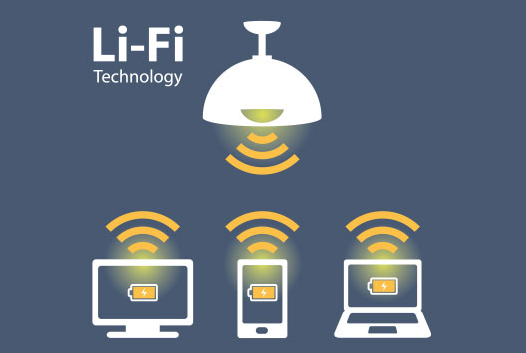
\includegraphics[width=80mm]{lifi.png}
    \caption{Tecnologia Li-Fi}
\end{figure}


\subsection*{Avantatges de Li-Fi}
\addcontentsline{toc}{subsection}{Avantatges de Li-Fi}

\subsubsection*{Sostenibilitat: menor cost i més eficiència}

Els seus avantatges no estan només a la velocitat. S'estima que en un futur proper podrem transmetre dades a través de l'energia solar, cosa que facilitarà l'accés a persones sense Internet i amb recursos d'electricitat limitats. El funcionament de la tecnologia Li-Fi estalviarà costos a les llars i, sobretot, als llocs de treball. Podria funcionar sense dispositius electrònics com ara rúters, mòdems, repetidors, amplificadors d'ona i antenes.

Aquests dispositius, que actualment estan connectats a la xarxa elèctrica les 24 hores del dia, els 7 dies de la setmana, deixarien de consumir electricitat i la seva funció seria reemplaçada per una bombeta LED, que en la majoria dels casos ja està encesa durant el horari de treball, per tant, no significaria un cost extra.

La principal diferència entre Li-Fi i altres formes de comunicació òptica, com ara la fibra òptica, és que Li-Fi no utilitza fils físics per a la transmissió de dades. En canvi, transmet les dades mitjançant la il·luminació LED ja existent en un entorn. Aquesta tecnologia pot oferir velocitats de transmissió de dades molt altes i també pot ser utilitzada en entorns on les comunicacions per ones de ràdio poden ser limitades, com ara en hospitals o en aules on l'ús de ones de ràdio pot estar restringit.

\subsubsection*{Seguretat contra atacs}

Com que cal estar en contacte directe amb l'emissor de feix de llum LED, es reforça la seguretat
informàtica. Només els dispositius il·luminats per la mateixa bombeta poden interconnectar-se entre si,
eliminant atacs o intents d'entrada no autoritzats des de dispositius fora del nostre espectre de
llum.
Una soluci´o brillant, més segura, més ràpida i eficient per optimitzar la nostra connexió amb el
món.


\subsection*{Incovenients de Li-Fi}
\addcontentsline{toc}{subsection}{Incovenients de Li-Fi}

Encara que la tecnologia Li-Fi ofereix algunes avantatges, també té alguns inconvenients i limitacions que poden afectar la seva adopció i implementació:


\begin{itemize}
    \item Dependència de la llum visible: La transmissió de dades a través de Li-Fi depèn de la llum visible, de manera que la comunicació pot veure afectada per la falta de llum, com en entorns foscos o quan les llums estan apagades.
    \item Limitacions d'abast: La cobertura de Li-Fi és generalment més limitada que la del Wi-Fi, ja que la llum no penetra a través de parets o altres obstacles com ho fa la radiació de radiofreqüència.
    \item Interferència de la llum solar: La llum solar pot interferir amb la transmissió de dades Li-Fi, ja que les dues fonts de llum poden ser captades pel receptor, provocant interferències i afectant el rendiment de la comunicació.
    \item Limitacions de mobilitat: La tecnologia Li-Fi pot ser menys adequada per a dispositius en moviment, ja que requereix una connexió visual constant amb la font de llum per a una transmissió de dades eficaç.
\end{itemize}








\subsection*{Wi-Fi vs Li-Fi}
\addcontentsline{toc}{subsection}{Wi-Fi vs Li-Fi}


\begin{table}[h]
\centering
\begin{tabular}{ | p{5.5em} | p{19em} | p{19em} | } 
\hline
 & Wi-Fi  (Wireless Fidelity)& Li-Fi  (Light Fidelity)\\
\hline
Avantatges & més interferència, no atraviesa l'aigua de mar, funciona en regions menys denses 
& menys interferència, pot atravesar l'aigua de mar, funciona en regions denses \\
\hline
Aplicació & S'utilitza per navegar per Internet amb l'ajuda de punts d'accés Wi-Fi 
& S'utilitza en aerolínies, exploracions submarines, quiròfans a hospitals, oficines i locals domèstics per a la transferència de dades i la navegació per Internet \\
\hline
Distancia de cobertura & uns 32 metres, varia segons la potència de transmissió i el tipus d'antena
& uns 10 metres \\
\hline
Densitat de dades & Funciona en entorns menys densos a causa de problemes relacionats amb la interferència 
& Funciona en entorns de alta densitat \\
\hline
Interferències & Diverses fonts d'interferències de ràdio poden interrompre el funcionament d'una xarxa Wi-Fi 
& No tenen problemes de interferència similar a les ones de radiofreqüència\\
\hline
Operació & Wi-Fi transmet dades utilitzant ones de radio amb l'ajuda d'un encaminador Wi-Fi
& LiFi transmet dades utilitzant fonts de llum (actualment focus LED) \\
\hline
Privacitat &  Wi-Fi és menys segur perquè el senyal no pot ser bloquejat per parets i la majoria dels objectes 
& Amb LiFi, les parets bloquegen la llum, i per tant, proporcionarà una transferència de dades més segura \\
\hline
\end{tabular}
\end{table}




\subsection*{Productes Li-Fi}
\addcontentsline{toc}{subsection}{Productes Li-Fi}

\subsubsection*{LiFiMAX Compact}

El LiFiMAX Compact és un sistema plug-and-play revolucionari que ofereix una connexió a Internet sense fils increïblement ràpida, segura i fiable a través de la llum invisible.


\begin{figure}[h!]
    \centering
    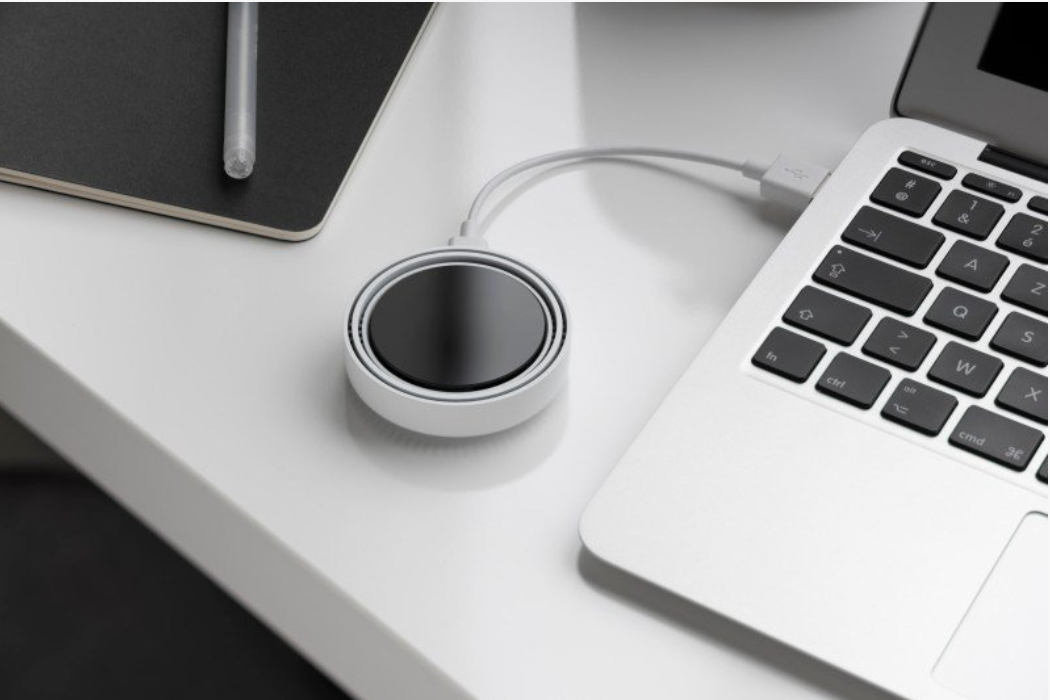
\includegraphics[width=80mm]{lifimaxaa.png}
    \caption{Li-Fi MAX}
\end{figure}

\subsubsection*{LiFiMAX Tab}

LiFiMAX Tab és una tauleta que es connecta a Internet mitjançant llum invisible. Aquesta tauleta és una alternativa revolucionària als dispositius actuals amb Wi-Fi. LiFiMAX Tab permet als usuaris connectar-se a través d'una connexió estable, ràpida i sense radiofreqüències que pot ser difícil d'interceptar fora de l'habitació. És perfecte per a l'ús de l'oficina a casa.

Sempre que es tingui antenes o punts d'accés LiFiMAX instal·lats a casa, es pot utilitzar LiFiMAX Tab amb facilitat. Ni tan sols es necessita un dongle per connectar-lo a Internet. Això fa que sigui més còmode d'utilitzar, sobretot si dos o tres membres de la família comparteixen la tauleta. 


\begin{figure}[h!]
    \centering
    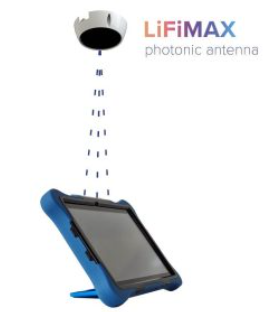
\includegraphics[width=40mm]{LiFiMAX.png}
    \caption{Li-FiMAX}
\end{figure}


\subsubsection*{MyLiFi lamp}

La làmpada MyLiFi és un llum d'escriptori amb una connectivitat LiFi segura, ràpida (23 Mb/s-) i sense ones de ràdio.

Les aplicacions mòbils i basades en web proporcionen control sobre la brillantor i la temperatura del color que van des del blanc càlid (2200K) fins a la llum del dia (6500K), permetent als usuaris crear el seu ambient preferit.


\begin{figure}[h!]
    \centering
    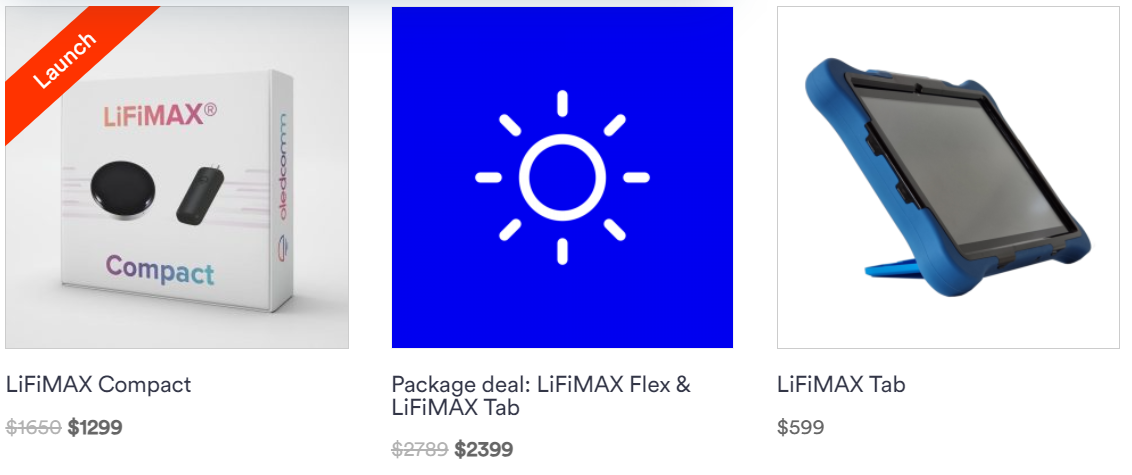
\includegraphics[width=80mm]{producteslifi.png}
    \caption{Altres productes Li-Fi i els seus preus}
\end{figure}


\section{Relacionar IEEE amb VLC}

\section{Conclusió}
\subsection*{A cares del futur}
\addcontentsline{toc}{subsection}{A cares del futur}

- poden juntar wifi+lifi


\section{Mercat futur de VLC}

\subsection*{Anàlisi de mercat VLC}
\addcontentsline{toc}{subsection}{Anàlisi de mercat VLC}

El mercat global de comunicacions de llum visible està valorat en 1.800 milions de dòlars l'any en curs i s'espera que registri un CAGR del 40,1\% durant el període de previsió, arribant als 19.300 milions de dòlars al final del període de previsió. La necessitat de transferència de dades d'alta velocitat, seguretat de dades, una imminent restricció de l'espectre de RF i diversos avantatges tecnològics sobre la tecnologia Wi-Fi impulsa principalment el mercat de la comunicació amb llum visible. A més de ser més rendible, Li-Fi té diversos avantatges respecte a la tecnologia Wi-Fi actual, com ara una velocitat de transferència de dades aproximadament 100 vegades més ràpida, una major seguretat de dades, cap interferència electromagnètica i un menor ús d'energia.


\begin{figure}[h!]
    \centering
    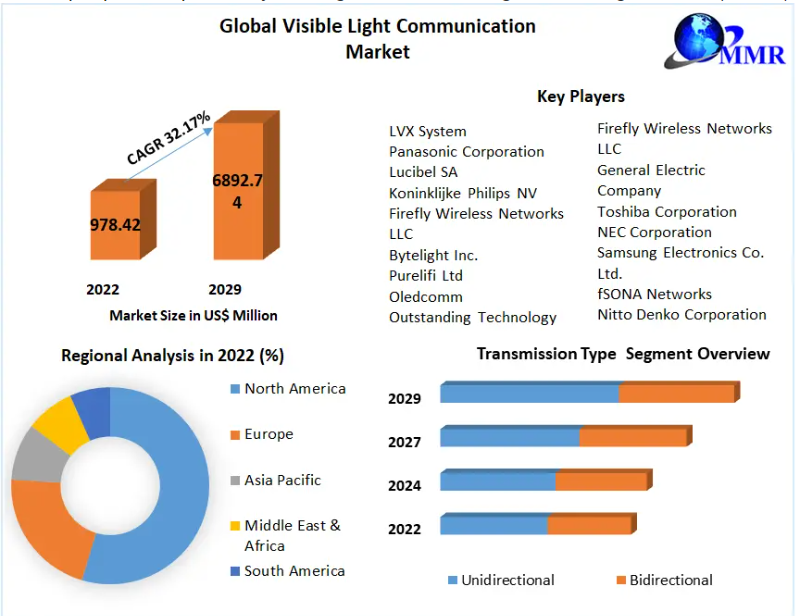
\includegraphics[width=80mm]{visiogeneralVLC.png}
    \caption{Mercat mundial del VLC }
\end{figure}



\subsection*{Tendències del mercat VLC}
\addcontentsline{toc}{subsection}{Tendències del mercat VLC}

\begin{itemize}
    \item Segons Ericsson, el nombre global de subscripcions a la xarxa mòbil de telèfons intel·ligents va superar els 6.600 milions el 2022 i s'espera que arribi als 7.800 milions el 2028. Els països amb més subscripcions a la xarxa mòbil de telèfons intel·ligents són la Xina, l'Índia i els Estats Units. Un augment tan gran dels telèfons intel·ligents crearia oportunitats lucratives per al mercat estudiat. 
    \item A més, s'esperava que les subscripcions mòbils 5G assoleixin aproximadament els 5.000 milions a finals de 2028. A més, es preveu que la cobertura de la població 5G arribi al 85\%, mentre que les xarxes 5G probablement portaran al voltant del 70\% del trànsit mòbil per al 2028. És probable que aquests esdeveniments també impulsin la demanda d'electrònica de consum, impulsant així el creixement del mercat estudiat. 
    \item Finalment, la popularitat dels dispositius domèstics intel·ligents està augmentant a mesura que els consumidors busquen maneres de fer que les seves cases siguin més còmodes, còmodes i segures. VLC pot controlar dispositius domèstics intel·ligents, cosa que la converteix en una tecnologia clau per al mercat.
\end{itemize}


\begin{figure}[h!]
    \centering
    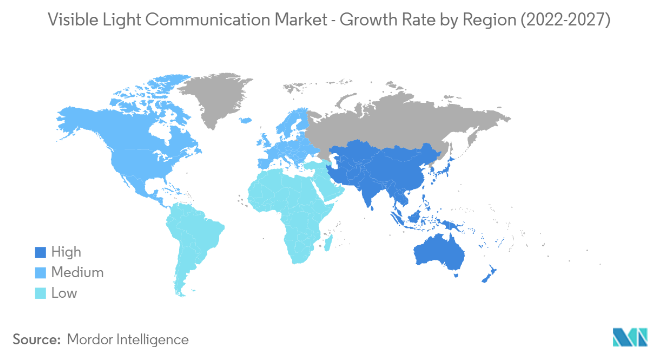
\includegraphics[width=80mm]{futurMundial.png}
    \caption{Amèrica del Nord comptarà amb la quota de mercat més gran}
\end{figure}









\clearpage

\section{Bibliografies}

https://openaccess.uoc.edu/bitstream/10609/95748/7/rarellanoTFG0619memoria.pdf

https://www.maximizemarketresearch.com/market-report/global-visible-light-communication-market/54383/
\clearpage

\end{document}